\documentclass[]{article}
\usepackage{tikz}
\usepackage{listings}


%opening
\title{A Theory of Micro Economic Behaviour}
\author{"The first draft of anything is shit."}


\begin{document}

\maketitle
\newpage

%\begin{abstract}
%\end{abstract}



\subsection{Context}

There pretext of this document is as  follows. Human behaviour as well as economics is difficult to predict due to factors such as scale, human variability in physical terms as well as the subjective nature of each individual. However at scale a model that can predict behaviour of the average individual is sufficient to use. The goal being that this could be used to understand and optimise ones own situation as well as attempt to forecast the short term future.

\subsection{Assertions}

The theory rests on the bases if these assertions;
\begin{enumerate}
  \item \textbf{\textit{That effort can be defined in this context as the the total integration of pain/pleasure that the subject experiences over a duration of time.}}
  \item \textbf{ \textit{That when a subject is presented with an opportunity of voluntary exchange that they will choose the option that minimises their own net effort.}}

\end{enumerate}

However since each person has different predispositions to what activities they like or don't like the amount of effort that should be attributed to that activity differs person to person. Since subjects are all unique it would be inappropriate make value proportional to simply the net effort associated with a good or service, as tempting as \textit{that} may be. Instead metrics of effort can only be used for comparing the same subject.  

Using these assumptions a model can be contracted. For instance the value of an itom 

made entirely by hand from a manufacturer, expludin the use of tools is the  from the persepective of the producer  to provide it to the providor and less 
than that of the next best opton to the recipiant.

When given the chance people will make volontary exchanges in order to reduce their total effort output. This 
exchange will be made if the option is of lower net effort than the next best option. 
People tend to arange all economic activity in turms of effort. 


Efficiently: typically in engineering no system can have an efficiency of more than 1, however in this context the $e$ acts as a coefficient of the $(\delta v output) / ( \delta v input)$. As sometimes storing things can add to the value it is possible to get more pleasure from it than was put in.

That there are only labour costs and nothing else. For example take any product or service, the price is defined as only the total of all labour coast associated with the product. in manufacturing a product is often broken down into labour costs and non-labour costs. Non-lobar costs often include materials, parts, tools, tool ware, tool depreciation and transport costs. I would like to assert that this may be true of the current level of manufacturing but not true when considering all layers of production. from example a product that is the comprised of a raw material and labour can be expressed as the sum of the labour of that processes as well as the labour involved in extracting and transporting the raw material. 

All claims made with respect to trading assume a free market.

\subsection{Definition of effort denoted by $\rho$, $\varphi$, $P$}
%can also do \subsubsection{Title}

at a fundamental level human interaction can be ranked on a scale of pleasure and pain. Henceforth denoted as $\rho$. This can be used to describe the pleasure of an event at an instant in time. similar to the concept of black body radiation the idea of there being a value of $\rho$ is absolute and is the identical scale between people. What does not remain constant is that two people may have two values of $\rho$ for the same activity as it's level of effect varies subjectively \\
\begin{figure}[!h]
	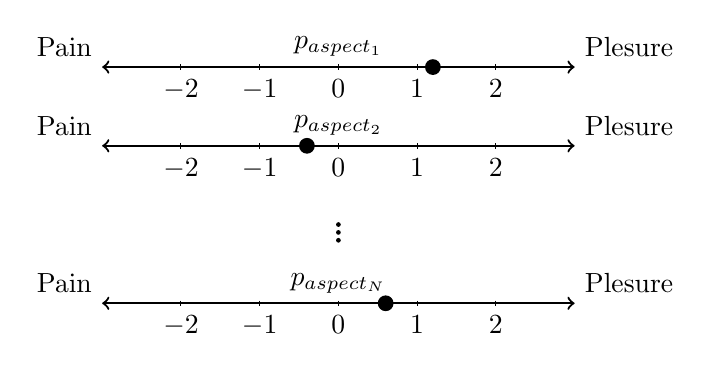
\begin{tikzpicture}
		\draw[thick] (0,1) -- (0,1) node[anchor=south]{$p_{aspect_{1}}$};
		\draw[thick,->] (0,1) -- (-3,1) node[anchor=south east]{Pain};
		\draw[thick,->] (0,1) -- (3,1) node[anchor=south west]{Plesure};
		\foreach \x in {-2,-1,0,1,2}
			\draw (\x cm,1pt + 1 cm) -- (\x cm,-1pt + 1 cm) node[anchor=north] {$\x$};
		\fill[black] (1.2, 1) circle (1mm);
		
		\draw[thick] (0,0) -- (0,0) node[anchor=south]{$p_{aspect_{2}}$};
		\draw[thick,->] (0,0) -- (-3,0) node[anchor=south east]{Pain};
		\draw[thick,->] (0,0) -- (3,0) node[anchor=south west]{Plesure};
		\foreach \x in {-2,-1,0,1,2}
			\draw (\x cm,1pt) -- (\x cm,-1pt) node[anchor=north] {$\x$};
		\fill[black] (-0.4,0) circle (1mm);
		
		\foreach \x in { 0, -0.1, -0.2}
			\fill[black] (0, \x - 1) circle (0.3mm);
			
		\draw[thick] (0,-2) -- (0,-2) node[anchor=south]{$p_{aspect_{N}}$};
		\draw[thick,->] (0,-2) -- (-3,-2) node[anchor=south east]{Pain};
		\draw[thick,->] (0,-2) -- (3,-2) node[anchor=south west]{Plesure};
		\foreach \x in {-2,-1,0,1,2}
			\draw (\x cm,1pt -2 cm) -- (\x cm,-1pt -2 cm) node[anchor=north] {$\x$};
	\fill[black] (0.6, -2) circle (1mm);
	\end{tikzpicture}
	\centering
\end{figure}
\\
The total of all pleasure and pain that an individual is experiencing at any one time is $P$ where:
\begin{equation}\label{Pdef}
	P = \sum \rho
\end{equation}
A scale of attributed pleasure value $\rho$ integrated over the time of an activity can be defined as the sum of the integrated change in pleasure with respect to that activity:
\begin{equation}\label{phidef}
	\varphi = \sum{\int{ \Delta \rho  \:  dt }}
\end{equation}
This can be thought of as a fundamental store input of value. Not necessarily the output of value ether. Since the exact scale of value for each individual is not represented in a standardised format translatable to another The effective of 'value' ($\varphi$). An efficient can only be meaningful in the context of the individual's 'value' spent to that of the potential 'value' returned.
\begin{equation}
	\eta = \frac{\varphi_{potentualOutput}}{\varphi_{input}} 
\end{equation} 
This value is not limited to the traditional domain of $\left\lceil 0, 1 \right\rceil $, instead being capable of residing at $>1$.



\subsection{Individual trade-off}
An individual will (generally) opt to choose the option at any time that is has the most $\varphi$, such as doing option $a$ or not doing option $a$. When ignoring time delay factors a trade for $a$ can be expressed as:
\begin{equation}\label{ind_trd}
	\varphi_{option} > \varphi_{alternative}
\end{equation}
However when time difference is relevant, the pleasure and pain become subject to the expected or anticipated $\varphi$. Notice that the factors subject to time also has an effect in relation to the decision to make a trade.
\begin{equation}\label{ind_trd_tm}
	\varphi_{anticipated} + \varphi_{timeSubdugation} > \varphi_{alternative}
\end{equation}


\subsection{Exchanges}
The first assumption that must be made here is that the individual scaling of $\rho$ remain independent from both parties exchanging any form of effort. If person one ($p1$) and person two ($p2$) each \textit{perceive} the exchange as being the higher $\varphi$ it in therefore deemed in each of their own individual interests.
\begin{equation}\label{trade_def}
	(\varphi_{p1, trade} > \varphi_{p1, noTrade}) \cup (\varphi_{p2, trade} > \varphi_{p2, noTrade})
\end{equation}\\
when given options of trades people will choose the option that has the highest increment of $\varphi$
\begin{equation}\label{trade_chc}
	rows
\end{equation}


\subsection{Methodology of Analysis}

\subsection{Trade and Exchange}

\subsection{Time Dependant Problems}

\subsection{Probability Dependant Problems}

\subsection{Examples in Business}

\subsection{Examples in Marketing}

\subsection{Governance and Involuntary Trading}
This section attempts to discuss the effects that non consensual trade (in the context of this paper) that is implicit in the role of government.

\subsection{Ethics}
Perhaps it is appropriate to include a section on the ethics of the types of dynamics at play discusses in these chapters. This is subject to the perspective of the reader as it is not uncommon for people to perceive situations in entirely different terms particularly when terms such as involuntary. However the perspective that this document seeks to put forward can shed some light on ethical conundrums. 

A criticism often levelled at ideologies that favour free trade or in more general terms larger degrees of purely voluntary exchange, is that advertising has a negative effect on the 


\end{document}


word graveyard

The distinction between the local coordinate $p$ and the global coordinate $P$ can be made by overlaying the scales of each individual definition of $p$ to the global scale for an activity. 



that relative value $\varphi$ can be defined numerically as the integral of  potential $p$ over time. where negative numbers represented discomfort two distinctions can be made. first that there is the $\varphi$' that is apparent from the amount of value that has gone into an activity. the second, the amount of value that has been saved by acquiring 'v' value. 'delta



the range of this scales $\left\lceil - \infty, \infty \right\rceil $. Where activities can have a $p$ value that changes over time. Due to how humans perceive meaning moralistically, an arbitrary scale can be assignment to this dimension as the most meaningful or pleasurable things will 'resize' the scale
